\section{Results}
\label{sec:results}

\subsection{The behavior exists and grows with scale}

\begin{table}[t]
    \centering
    \caption{Baseline sycophancy on the 240 evaluation items. All four models choose the sycophantic answer more often than the 50\% expected without sycophancy, and both the rate and the logit margin grow with model size.}
    \label{tab:baseline}
    \small
    \begin{tabular}{@{}lccc@{}}
        \toprule
        \textbf{Model} & \textbf{Greedy sycophantic rate (95\% CI)} & \textbf{$p$ vs.\ 50\%} & \textbf{Mean logit margin} \\
        \midrule
        0.5B & 0.588 (0.522--0.650) & 0.008 & 0.44 \\
        1.5B & 0.767 (0.708--0.819) & $<0.001$ & 1.50 \\
        3B & 0.883 (0.836--0.921) & $<0.001$ & 7.64 \\
        7B & 0.929 (0.889--0.958) & $<0.001$ & 13.45 \\
        \bottomrule
    \end{tabular}
\end{table}

\Tabref{tab:baseline} shows that all four models are sycophantic at baseline.
The greedy sycophantic-answer rate rises from 0.588 at 0.5B to 0.929 at 7B, and the mean logit margin rises from 0.44 to 13.45.
The 0.5B model is close to chance on two of the three domains (0.54 on NLP survey and 0.48 on political typology), so it offers little behavior to reduce.
We keep it in the map because a weak baseline is itself a common source of nulls.

\subsection{The map: nulls form vertical bands}

\begin{figure}[t]
    \centering
    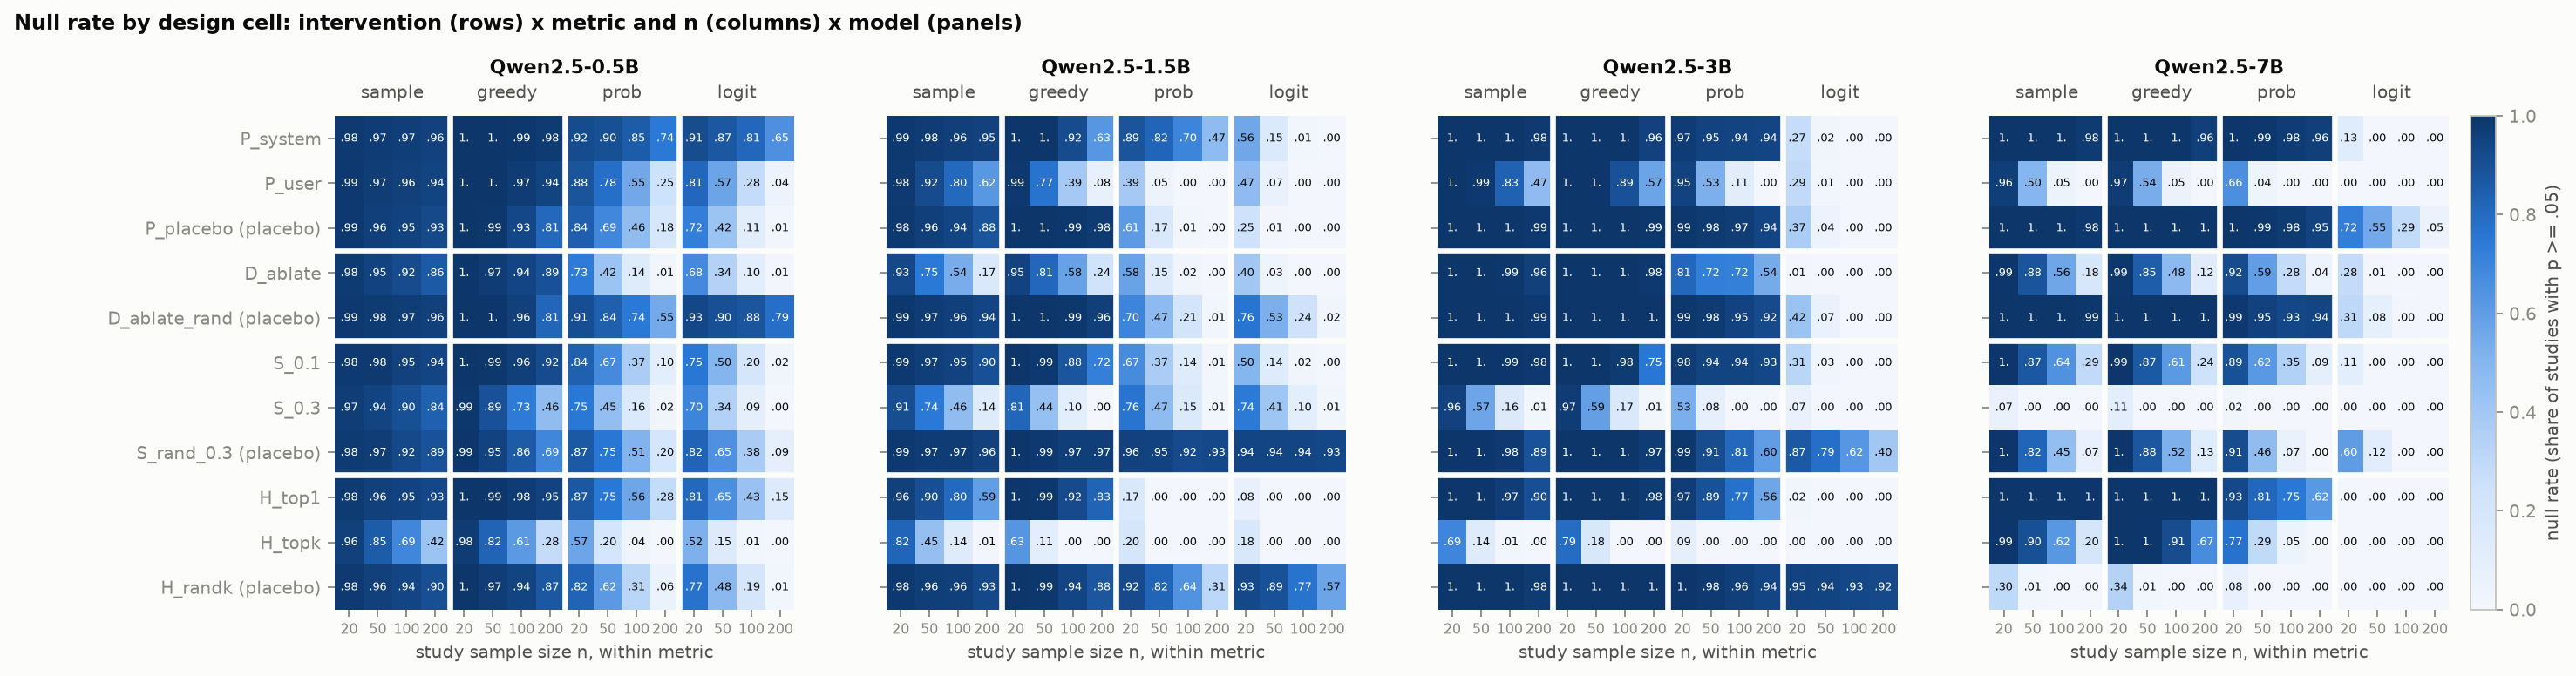
\includegraphics[width=\linewidth]{figures/fig1_null_map.png}
    \caption{Null rate for all 704 design cells. Rows are interventions, panels are models, and columns are metrics, each split into four sample sizes. Dark cells are designs where almost every study returns $p \ge .05$. The dominant pattern is vertical: for the same row, the \msample and \mgreedy columns are mostly dark and the \mlogit columns mostly light.}
    \label{fig:map}
\end{figure}

\Figref{fig:map} shows the full map.
The overall null rate is 0.59, and 0.52 when we exclude placebos.
The picture is dominated by vertical bands.
Within a row, where the model, the intervention, and the items are fixed, the left half of each panel (\msample, \mgreedy) is mostly dark and the right edge (\mlogit) is mostly light.
Horizontal structure, which would indicate that some interventions or granularities yield nulls regardless of metric, is much weaker.

\subsection{Metric and sample size organize the nulls; granularity and scale do not}

\begin{table}[t]
    \centering
    \caption{Marginal null rates by design feature, with 95\% cluster-bootstrap CIs over the 44 units. The lowest null rate in each row is in \textbf{bold}. The smallest $p$-value that 5000 permutations can produce is 0.0002. The last column gives each feature's share of cell-level variance in null rate.}
    \label{tab:marginals}
    \resizebox{\textwidth}{!}{%
    \begin{tabular}{@{}lccccc@{}}
        \toprule
        \textbf{Feature} & \multicolumn{4}{c}{\textbf{Null rate by level (95\% CI)}} & \textbf{Test; variance share} \\
        \midrule
        \multirow{2}{*}{Metric} & \msample & \mgreedy & \mprob & \mlogit & \multirow{2}{*}{$p = 0.0002$; 32\%} \\
         & 0.81 (0.73--0.88) & 0.80 (0.71--0.87) & 0.52 (0.42--0.62) & \textbf{0.25} (0.17--0.34) & \\
        \midrule
        \multirow{2}{*}{Sample size} & $n=20$ & $n=50$ & $n=100$ & $n=200$ & \multirow{2}{*}{$p = 0.0002$; 10\%} \\
         & 0.77 (0.71--0.83) & 0.64 (0.56--0.71) & 0.53 (0.45--0.61) & \textbf{0.43} (0.35--0.52) & \\
        \midrule
        \multirow{2}{*}{Granularity} & prompt & all layers & single layer & head & \multirow{2}{*}{$p = 0.88$; 2\%} \\
         & 0.66 (0.54--0.76) & 0.65 (0.53--0.76) & 0.56 (0.41--0.70) & \textbf{0.53} (0.35--0.68) & \\
        \midrule
        \multirow{2}{*}{Model} & 0.5B & 1.5B & 3B & 7B & \multirow{2}{*}{descriptive; 5\%} \\
         & 0.70 (0.62--0.78) & 0.55 (0.42--0.68) & 0.65 (0.49--0.79) & \textbf{0.47} (0.30--0.63) & \\
        \bottomrule
    \end{tabular}}
\end{table}

\begin{figure}[t]
    \centering
    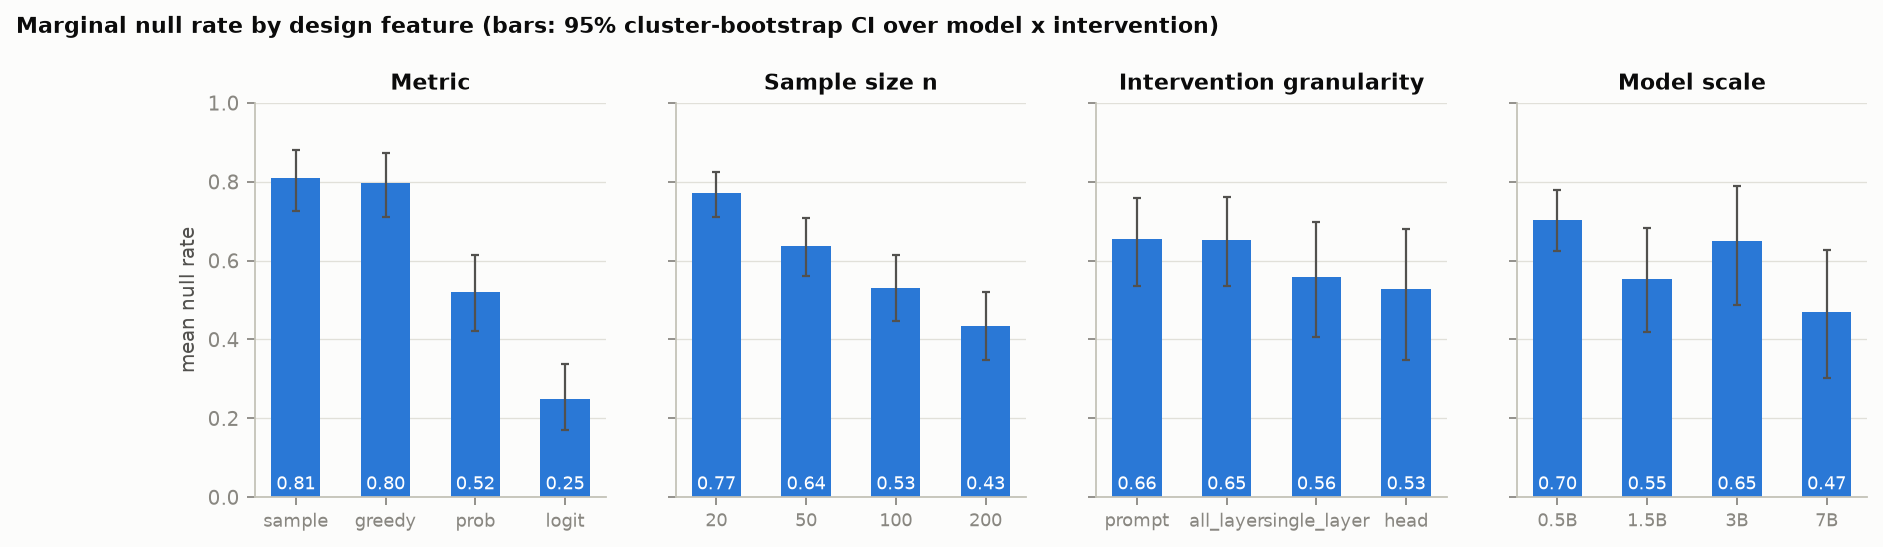
\includegraphics[width=\linewidth]{figures/fig2_marginal_null_rates.png}
    \caption{Marginal null rate by design feature. Error bars are 95\% cluster-bootstrap CIs over model--intervention units. Null rate falls steeply from answer-level to logit-level metrics and with sample size. Differences between granularities and between models are small relative to their intervals.}
    \label{fig:marginals}
\end{figure}

\para{H1 (metric) is supported.}
\Tabref{tab:marginals} and \figref{fig:marginals} show the marginal null rates.
The null rate is 0.81 for \msample and 0.80 for \mgreedy, falls to 0.52 for \mprob, and to 0.25 for \mlogit.
The range across metrics is 0.56 (permutation $p = 0.0002$).
The ordering is the same when we exclude placebos (0.76, 0.74, 0.44, 0.15) and at $\alpha = .01$ (0.87, 0.86, 0.64, 0.34).

\para{Sample size matters, but less than metric.}
The null rate falls from 0.77 at $n = 20$ to 0.43 at $n = 200$, a range of 0.34 ($p = 0.0002$).
A tenfold increase in items therefore buys less than switching from an answer-level metric to the logit margin.

\para{H2 (granularity) is not supported.}
Null rates by granularity range from 0.53 for head-level to 0.66 for prompt-level interventions, and a permutation test over intervention labels gives $p = 0.88$ ($p = 0.90$ without placebos).

\para{H3 (scale) shows no monotone trend.}
Null rates are 0.70, 0.55, 0.65, and 0.47 from the smallest to the largest model.
The 7B model has the lowest rate and the 0.5B model the highest, but the 3B model sits above the 1.5B model and the intervals overlap widely.

\para{Variance shares.}
In a descriptive decomposition of null rate across the 704 cells, metric accounts for 32\% of the variance, sample size for 10\%, model for 5\%, and granularity for 2\% ($R^2 = 0.48$).
Adding the reference effect size raises $R^2$ to 0.64 and leaves the metric and sample-size shares unchanged.
The remaining 36\% is specific to individual model--intervention pairs.

\subsection{Reference effects: logit shifts are nearly universal, answer changes are not}

\begin{figure}[t]
    \centering
    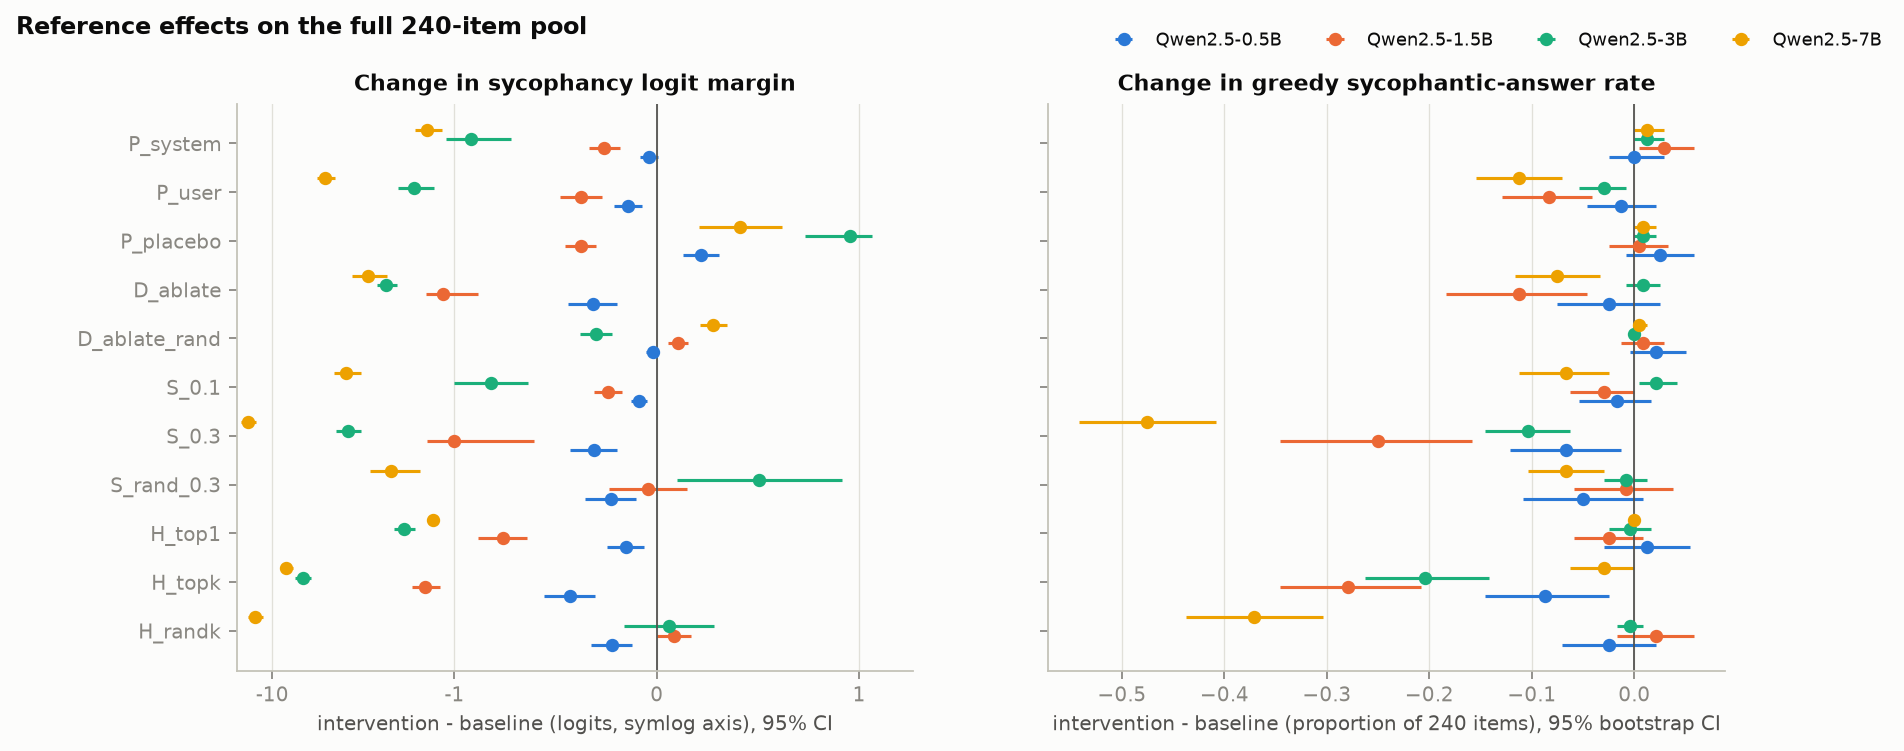
\includegraphics[width=\linewidth]{figures/fig3_reference_effects.png}
    \caption{Reference effects on the full 240-item pool. \figleft Change in the sycophancy logit margin (symmetric log axis). \figright Change in the greedy sycophantic-answer rate. Most interventions move the logit margin away from zero with tight intervals, while most changes in answer rate are within a few points of zero. On 7B, the placebo \intv{H\_randk} has one of the largest effects in the study.}
    \label{fig:reference}
\end{figure}

Of the 44 units, 10 are \behav, 28 are \latent, and 6 are \noeff.
Among the 28 non-placebo units the counts are 8, 19, and 1; the single \noeff unit is \intv{P\_system} on 0.5B.
\Figref{fig:reference} shows the effects, and \tabref{tab:reference_full} in the appendix lists every unit.
Three observations matter for interpreting the map.

\para{Logit shifts are common and answer changes are rare.}
Of the 28 non-placebo interventions, 27 shift the logit margin and 8 change the greedy answer rate.

\para{Placebos are not inert.}
Of the 16 placebo units, 11 have a detectable effect and 2 are \behav.
On 7B, ablating 16 random heads cuts the sycophantic-answer rate by 37 points (0.93 to 0.56), far more than ablating the 16 attribution-selected heads (3 points).
The attribution-based selection therefore did not find the most relevant heads on 7B, and placebo null rates are not a clean false-positive baseline.

\para{Metrics can disagree in sign.}
In 6 non-placebo units the mean logit margin falls while the greedy sycophantic rate rises slightly.
These include \intv{P\_system} on 1.5B, 3B, and 7B.
On 1.5B, for example, the anti-sycophancy system prompt lowers the mean margin by 0.26 logits, yet it flips 2 answers away from sycophancy and 9 toward it.
None of these greedy changes is significant, but they show that a logit-level effect does not guarantee an answer-level effect in the same direction.

\subsection{What the nulls are made of}
\label{sec:composition}

\begin{table}[t]
    \centering
    \caption{Composition of nulls from non-placebo interventions, by reference class of the intervention. CIs are from a cluster bootstrap over units. The pre-specified criterion for ``blind spot'' was that most nulls fall in \behav units; the largest share (in \textbf{bold}) instead falls in \latent units.}
    \label{tab:composition}
    \small
    \begin{tabular}{@{}lccc@{}}
        \toprule
        \textbf{Reference class} & \textbf{Units} & \textbf{Share of nulls (95\% CI)} & \textbf{Mean null rate in class} \\
        \midrule
        \behav: answers change & 8 & 0.14 (0.05--0.27) & 0.25 \\
        \latent: logits shift, answers do not & 19 & \textbf{0.80} (0.62--0.93) & 0.62 \\
        \noeff: no detectable effect & 1 & 0.06 (0.00--0.19) & 0.91 \\
        \bottomrule
    \end{tabular}
\end{table}

\begin{figure}[t]
    \centering
    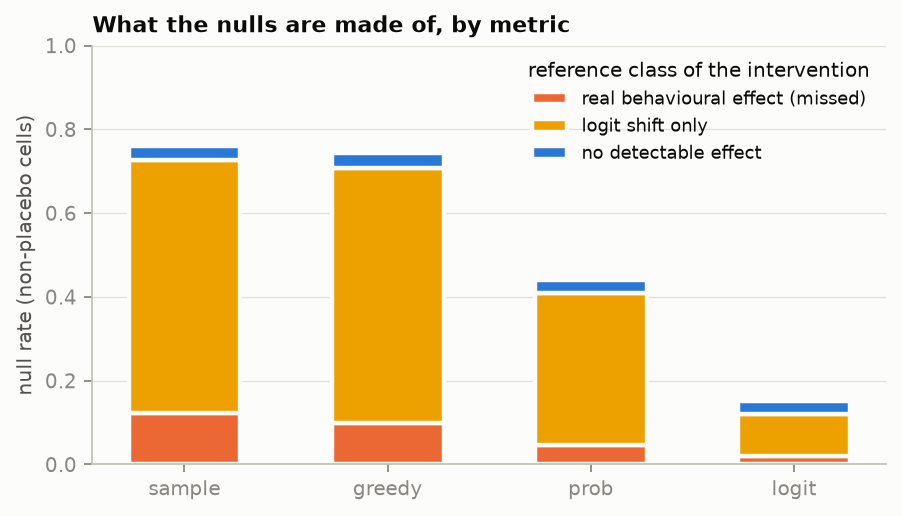
\includegraphics[width=0.62\linewidth]{figures/fig5_null_composition.png}
    \caption{Null rate in non-placebo cells by metric, split by the reference class of the intervention. For every metric, most nulls sit on interventions that shift logits without changing answers. Missed behavioral effects are a minority throughout.}
    \label{fig:composition}
\end{figure}

\para{H4 (blind spot) is not supported as pre-specified.}
\Tabref{tab:composition} shows where non-placebo nulls fall.
Only 14\% (95\% CI 5--27\%) fall on \behav interventions.
The large majority, 80\% (62--93\%), fall on \latent interventions, and 6\% fall on the one intervention with no detectable effect.
\Figref{fig:composition} shows the same split for each metric.
The \behav share is 0.10 when we exclude $n = 20$, 0.17 at $\alpha = .01$, and between 0.11 and 0.16 within each metric.

\para{Sensitivity to the classification threshold.}
The classification depends on the Holm threshold.
Five further non-placebo units have a greedy change with unadjusted $p < .05$; for example, \intv{D\_ablate} on 1.5B reduces the sycophantic rate by 11 points with Holm-adjusted $p = 0.12$.
Counting those five as \behav raises the share to 0.30.
This analysis is exploratory, and the share remains a minority.

\begin{table}[t]
    \centering
    \caption{Null rate in the 10 \behav units, where the intervention does change answers. Each entry is the probability that a study of that design misses a real behavioral effect. The lowest rate in each column is in \textbf{bold}.}
    \label{tab:missed}
    \small
    \begin{tabular}{@{}lcccc@{}}
        \toprule
        \textbf{Metric} & $n=20$ & $n=50$ & $n=100$ & $n=200$ \\
        \midrule
        \msample & 0.77 & 0.50 & 0.26 & 0.10 \\
        \mgreedy & 0.76 & 0.44 & 0.17 & 0.03 \\
        \mprob & 0.45 & 0.17 & 0.05 & 0.01 \\
        \mlogit & \textbf{0.23} & \textbf{0.06} & \textbf{0.01} & \textbf{0.00} \\
        \bottomrule
    \end{tabular}
\end{table}

\para{When a behavioral effect exists, the metric decides how often it is missed.}
\Tabref{tab:missed} restricts the map to \behav units.
At $n = 50$, a study that scores the greedy answer misses a real behavioral change 44\% of the time, and a study that scores the logit margin misses it 6\% of the time.
A logit-margin study with 20 items (0.23) is about as sensitive as a greedy-answer study with 100 items (0.17).
In \latent units the contrast is sharper: a greedy study is null 80--100\% of the time at any $n$, while a logit study at $n = 100$ is null 8\% of the time.

\begin{figure}[t]
    \centering
    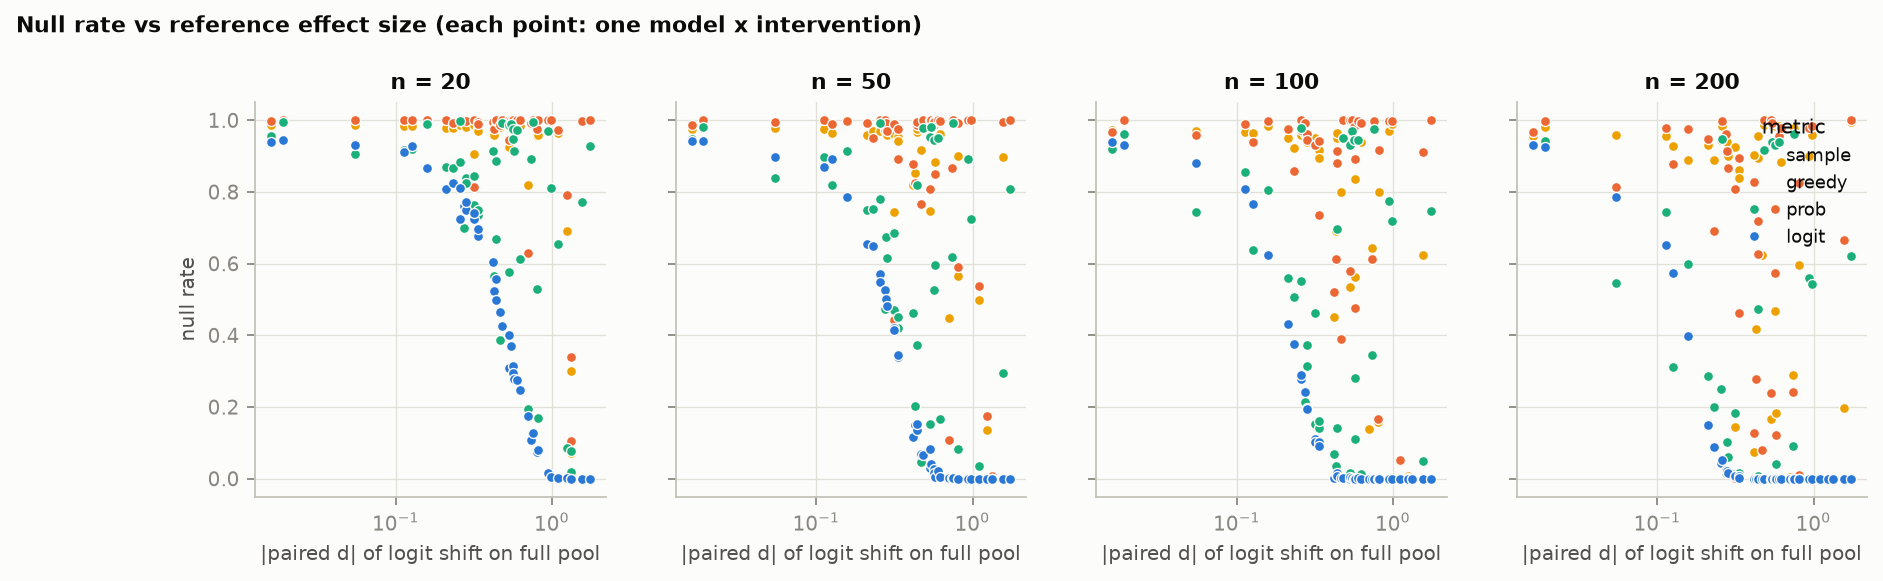
\includegraphics[width=\linewidth]{figures/fig4_null_vs_effect_size.png}
    \caption{Null rate against the reference effect size (absolute paired $d$ of the logit shift), one point per unit and metric, by sample size. For the \mlogit metric the null rate falls along a clean power curve. For answer-level metrics it stays near 1 for many units with large logit-level effects.}
    \label{fig:effectsize}
\end{figure}

\Figref{fig:effectsize} plots null rate against the reference effect size.
The \mlogit points trace a power curve, as expected for a $t$-test on the quantity that defines the effect size.
The answer-level points do not: many units with a standardized logit shift above 0.5 still return a null on \msample or \mgreedy in nearly every study.

\subsection{Metric by scale (exploratory)}

\begin{table}[t]
    \centering
    \caption{Null rate for non-placebo interventions by model and metric. The gap between \mgreedy and \mlogit is widest in the two larger models (in \textbf{bold}). This analysis was not planned and rests on four models.}
    \label{tab:metric_model}
    \small
    \begin{tabular}{@{}lccccc@{}}
        \toprule
        \textbf{Model} & \msample & \mgreedy & \mprob & \mlogit & \mgreedy $-$ \mlogit \\
        \midrule
        0.5B & 0.92 & 0.90 & 0.49 & 0.41 & 0.49 \\
        1.5B & 0.73 & 0.63 & 0.25 & 0.14 & 0.50 \\
        3B & 0.77 & 0.78 & 0.57 & 0.04 & \textbf{0.74} \\
        7B & 0.63 & 0.66 & 0.45 & 0.02 & \textbf{0.64} \\
        \bottomrule
    \end{tabular}
\end{table}

Although scale has no monotone effect on the overall null rate, \tabref{tab:metric_model} suggests that it changes how much the metric matters.
In the 3B and 7B models, logit-level studies almost never return a null (0.04 and 0.02), while answer-level studies usually do (0.78 and 0.66 for \mgreedy).
The baseline margins offer a plausible reason.
At 7.6 and 13.5 logits, a shift of 1--3 logits is easy to detect and cannot flip an answer held by that margin.
We did not plan this test, and scale is confounded with baseline sycophancy strength, so we treat this explanation as a hypothesis.
